\documentclass{exam}
\usepackage{graphicx}
\graphicspath{ {images/} }
\usepackage[utf8]{inputenc}

\title{Fall 2017 14.01 Problem Set 4}
\author{Robert Durfee}
\date{October 27, 2017}

\begin{document}

\maketitle

\section*{Problem 1}

\begin{enumerate}

\item \textbf{False}. If the supply is perfectly inelastic, then the total surplus will not decrease, there will only be an increase in consumer surplus and a decrease in producer surplus.

\item \textbf{False}. In inelastic conditions, a non-discriminating, profit-maximizing monopoly cannot choose an optimal price and quantity because marginal revenue is negative. A firm will not choose to produce if it will cause a loss of revenue.

\item \textbf{False}. All consumers are strictly worse off if the monopoly practices perfect price discrimination. All the surplus is for the producer and the consumers receive zero surplus. Each consumer pays their willingness to pay.

\item \textbf{False}. The total welfare will remain the same, but the consumer surplus will decrease and producer surplus will increase as the two groups are paying closer to their willingness to pay.

\end{enumerate}

\section*{Problem 2}

\begin{enumerate}

    \item Supply and demand functions for gasoline:
        \[D(P)=100-P\]
        \[S(P)=3P\]
        Set quantities equal to solve for equilibrium price:
        \[100-P^{*}=3P^{*}\]
        \[100=4P^{*}\]
        \[P^{*}=\mathbf{25}\]
        Substitute equilibrium price into demand function to solve for equilibrium quantity:
        \[Q^{*}=100-P^{*}\]
        \[Q^{*}=\mathbf{75}\]
        Find area under demand curve and above price to calculate consumer surplus:
        \[\int_{0}^{75} \left[(100-Q')-25\right] dQ'=\mathbf{2812.5}\]
        Find area above supply curve and under price to calculate producer surplus:
        \[\int_{0}^{75} \left[25-\frac{Q'}{3}\right] dQ'=\mathbf{937.5}\]
        Total surplus is the sum of both consumer and producer surplus:
        \[2812.5+937.5=\mathbf{3750}\]
    
    \item New equilibrium price is the price minimum \(\overline{P}\) as it is above the natural equilibrium:
        \[P^{*}=\mathbf{30}\]
        Substitute equilibrium price into demand function to solve for equilibrium quantity (as producers can't force consumers to purchase higher quantity):
        \[Q^{*}=100-P^{*}\]
        \[Q^{*}=\mathbf{70}\]
        Find area under demand curve and above price to calculate consumer surplus:
        \[\int_{0}^{70} \left[(100-Q')-30\right] dQ'=\mathbf{2450}\]
        Find area above supply curve and under price to calculate producer surplus:
        \[\int_{0}^{70} \left[30-\frac{Q'}{3}\right] dQ'=\mathbf{1283.3}\]
        Total surplus is the sum of both consumer and producer surplus:
        \[2450+1283.3=\mathbf{3733.3}\]
        Because the consumer surplus decreases, consumers are worse off. Because the producer surplus increases, the producer is better off. However, there is a decrease of \(16.7\) in total surplus as there are trades that could have been made where the producer was willing to sell a higher quantity at a lower price. This loss of trades results in a dead weight loss.
        
    \item The new equilibrium price and quantity will be the same because \(\overline{Q}=Q^{*}\) from the last answer:
        \[P^{*}=\mathbf{30}\]
        \[Q^{*}=\mathbf{70}\]
        The results obtained from a quota are the same as a price floor (so long as the quantity and price correspond to the same equilibrium position).
        
    \item Knowing that the firm's marginal cost is equal to market price, an increase of \(x\) can be shown:
        \[P=\frac{Q}{3}+x\]
        Rearranging this we can find the new supply curve:
        \[S(P)=3(P-x)\]
        Substitute our price floor/quota equilibrium as the natural equilibrium and solve for \(x\):
        \[Q^{*}=3(P^{*}-x)\]
        \[70=3(30-x)\]
        \[\frac{20}{3}=\mathbf{6.7}\]
        An increase of \$6.67 in input prices will result in a natural equilibrium at the price floor/quota.
        
\end{enumerate}

\section*{Problem 3}

\begin{enumerate}

    \item Calculate the expected value of the stock for each opportunity:
        \[E_{A}(y)=1.00\cdot102=\mathbf{102}\]
        \[E_{B}(y)=0.90\cdot0+0.10\cdot1000=\mathbf{100}\]
        \[E_{C}(y)=0.50\cdot90+0.50\cdot200=\mathbf{145}\]
        The maximum expected value is given through \textbf{Opportunity C}.
        
    \item Calculate the expected value of Mr. Cook's compensation from a stock:
        \[E_{A}(y)=1.00(102-100)=\mathbf{2}\]
        \[E_{B}(y)=0.90(0-100)+0.10(1000-100)=\mathbf{0}\]
        \[E_{C}(y)=0.50(90-100)+0.50(200-100)=\mathbf{45}\]
        Mr. Cook will choose \textbf{Opportunity C} which maximized his expected compensation.
        
    \item Calculate the expected value of Mr. Cook's compensation from a stock call option:
        \[E_{A}(y)=1.00(102-100)=\mathbf{2}\]
        \[E_{B}(y)=0.90\cdot0+0.10(1000-100)=\mathbf{90}\]
        \[E_{C}(y)=0.50\cdot0+0.50(200-100)=\mathbf{50}\]
        Mr. Cook will choose \textbf{Opportunity B} which maximizes his expected compensation, but does not maximize the expected value of Apple's stock.
        
    \item \textbf{Pros for stocks}:
        \begin{itemize}
            \item Manager's best interest will align with shareholders'.
        \end{itemize}
        \textbf{Cons for stocks}:
        \begin{itemize}
            \item Expensive for shareholders.
            \item Manager could turn around and sell stock immediately effectively making the stock a cash bonus.
        \end{itemize}
        \textbf{Pros for stock options}:
        \begin{itemize}
            \item Manager's best interest will often align with shareholders'.
            \item Less expensive than stock. 
            \item Manager can't turn around and sell the stock immediately.
        \end{itemize}
        \textbf{Cons for stock options}:
        \begin{itemize}
            \item On riskier choices, the manager's best interest does not align with shareholders' and gambling will often result.
            \item Stock options could be backdated effectively creating a larger reward.
        \end{itemize}
    
\end{enumerate}

\section*{Problem 4}

\begin{enumerate}

    \item Price elasticity of demand is defined as:
        \[E_{D}(P)=\frac{dQ_{D}}{dP}\frac{P}{Q_{D}}\]
        Substituting in the demand function:
        \[E_{D}(P)=\frac{d}{dP}(P^{-\epsilon})\frac{P}{P^{-\epsilon}}\]
        \[E_{D}(P)=-\epsilon P^{-\epsilon-1}P^{1+\epsilon}\]
        \[E_{D}(P)=\mathbf{-\epsilon P}\]
        
    \item Monopoly profit maximization condition:
        \[\max_{P} P D(P)-C(D(P))\]
        \[D(P)+P D'(P)-C'(D(P))D'(P)=0\]
        Substituting our demand and cost functions:
        \[P^{-\epsilon}+P(-\epsilon P^{-\epsilon-1})-(P^{-\epsilon})(-\epsilon P^{-\epsilon-1})=0\]
        Solving for P:
        \[\mathbf{P=\left(\frac{-\epsilon}{1-\epsilon}\right)^{1/(-\epsilon-1)}}\]
        
    \item Price markup for monopolies:
        \[P_{m}=-\frac{1}{E_{D}}\]
        Substituting our price elasticity of demand:
        \[P_{m}=\frac{1}{\epsilon P}\]
        Substituting our optimal price:
        \[\mathbf{P_{m}=\frac{1}{\epsilon}\left(\frac{1-\epsilon}{-\epsilon}\right)^{1/(-\epsilon-1)}}\]
        Price markup for \(\epsilon=2\):
        \[\mathbf{P_{m}=0.63}\]
        Price markup for \(\epsilon=3\):
        \[\mathbf{P_{m}=0.37}\]
        As epsilon increases, the elasticity of demand increases. As a result, the demand curve becomes more horizontal. Although the firm has no competition for that particular good, there are other goods and therefore the markup has to decrease to represent the substitutability of different goods.
        
    \item Producer surplus: green shaded area. Consumer surplus: orange shaded area. Deadweight loss: purple shaded     area.\\
        Marginal cost: green curve. Marginal revenue: orange curve. Demand: red curve.\\\\
        \begin{center}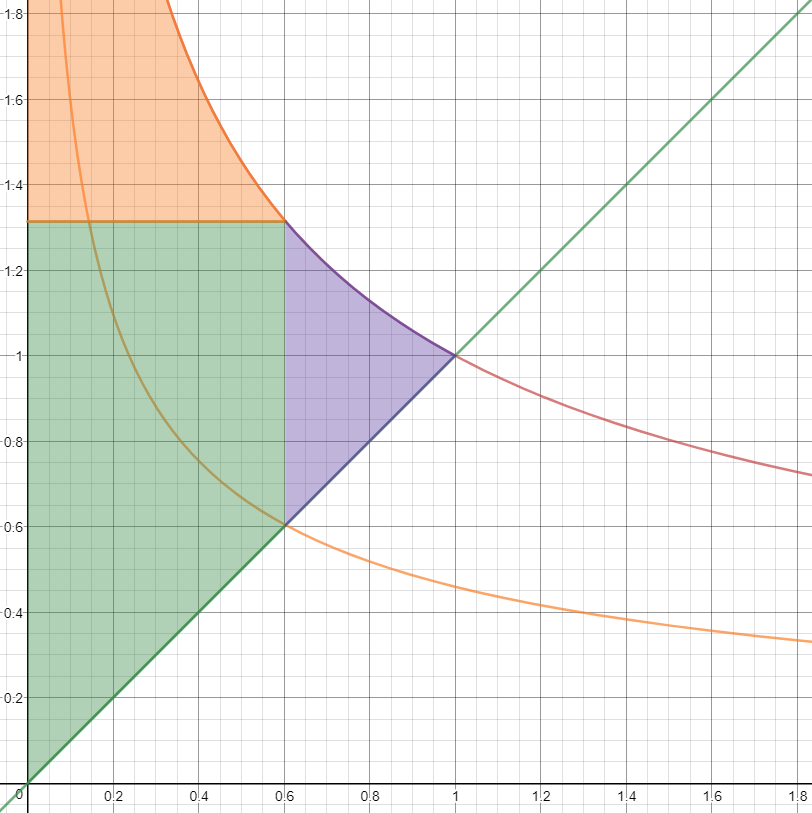
\includegraphics[scale=0.75]{Capture}\end{center}
        Horizontal axis: quantity, vertical axis: price.
    
\end{enumerate}
        
\end{document}
